\newpage

\subsection{Registracion y Ingreso al casino online y modificacion de saldo}

\subsubsection{Registracion}
Segun lo acordado, la registracion de los usuarios de hace por fuera del sistema informatico del casino online. Explicaremos como esperamos que interactuen los agentes externos para que el sistema posea la lista actualizada de usuarios registrados. Para ello usaremos el Diagrama de Activdades\footnote{Diagrama de Actividades: Grafico que representa el flujo de actividades. Las cajas representan actividades y las flechas repersentan secuencialidad y los rombos representan decisiones} ``Registracion''. Ver Figura: \ref{fig:daReg}

\begin{figure}[h!]
	\centering
		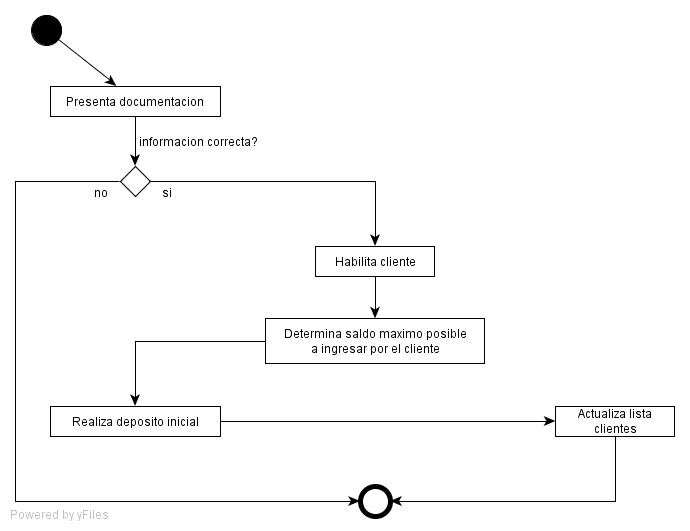
\includegraphics[scale=0.5]{img/daRegistracion.png}
	\caption{Diagrama de actividades Registracion\label{fig:daReg}}
\end{figure}

\textcolor{red}{falta nombre de responsables}

Cabe aclarar que el cliente podra comenzar a jugar en el casino recien cuando el casino se vuelva a abrir

\subsubsection{Modificacion de saldo}

Una vez registrado un cliente puede ingresar y retirar dinero real, dicha operacion solo podra realizarse mistras el casino permanece cerrado.
Explicaremos esta operatoria con un diagrama de actividades. Ver Figura: \ref{fig:modSaldo}

\begin{figure}[h!]
	\centering
		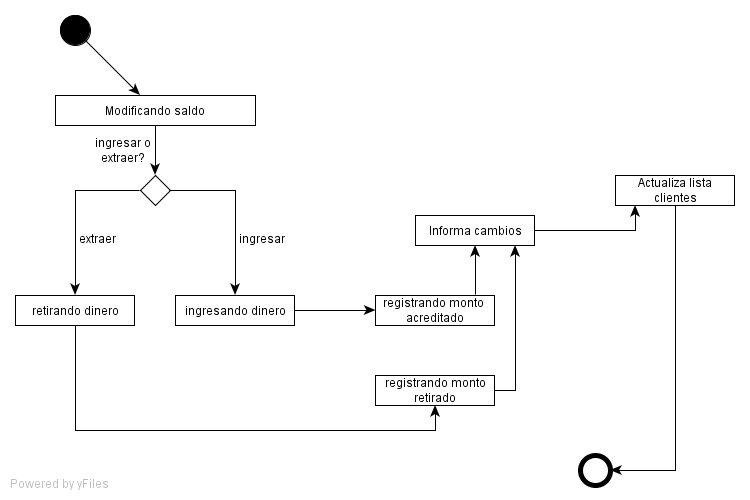
\includegraphics[scale=0.5]{img/clienteModSaldo.png}
	\caption{Diagrama de actividades Modificacion de Saldo\label{fig:modSaldo}}
\end{figure}

\textcolor{red}{falta nombre de responsables}

\subsubsection{Ingreso y egreso del casino}

La forma en que un cliente ingresa o egresa del casino esta explicado en los casos de uso: \\
CU \ic \ref{lic} y CU \salc \ref{lsalc}.

\subsection{Administracion del Casino}

\subsubsection{Apertura del casino}

En el momento de la apertura del casino es podible realizar configuraciones distintos aspectos:
\begin{itemize}
	\item Configuracion de valores de fichas
	\item Asignacion de probablilidades
	\item valores minimos para la entrega de premios
\end{itemize}

Dicha interaccion con el sistema esta explicada en el caso de uso: CU \ac \ref{lac}

\subsubsection{Clausura del casino}

La operatioria de cerrar el casino no es muy complicada, pero tiene una salvedad. No es posible cerrar el casino si hay jugadores dentro del casino

Dicha interaccion con el sistema esta explicada en el caso de uso: CU \ccas \ref{lccas}

\begin{framed}

\depto Con esta maquina de estados finitos (FSM) Mostramos que nos comprometemos a que un administrador podr� cerrar el casino solo si no hay ningun cliente en el mismo.


{\large FSM: Administrador}
\begin{center}
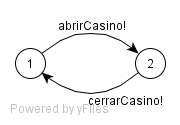
\includegraphics[scale=0.5]{img/admin.png}
\end{center}


{\large FSM: Jugador$_i$}
\begin{center}
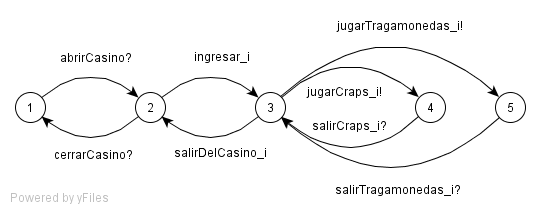
\includegraphics[scale=0.5]{img/jugador.png}
\end{center}

\end{framed}

\subsection{Modo Dirigido}

\subsubsection{Inicio de Modo Dirigido}

Cuando se ingresa en este modo, los resultados de las jugadas no seran al azar sino que el manipulador decidira los mismos.

Esos resultados ingresados se respetaran para todas las jugadas de todas las mesas habilitadas de ese juego mientras no se vuelva a modo normal.

Dicha interaccion con el sistema esta explicada en el caso de uso: CU \actm \ref{lactm}
\begin{framed}

\depto Con esta maquina de estados finitos (FSM) Mostramos que en modo dirigido se pueden lanzar jugadas de forma manual, dicha funcionalidad no esta permitida en modo normal.
Es seteo de las jugadas debe hacerse en el momento de entrar en modo dirigido. 

\paragraph{FSM: Administrador}
\begin{center}
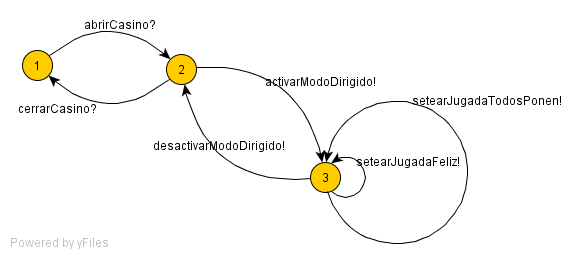
\includegraphics[scale=0.5]{img/manipulador.png}
\end{center}

\end{framed}

\subsubsection{Seteo de Jugadas Feliz y Todos Ponen}

El manipulador puede iniciar una Jugada Feliz, al hacerlo debe seleccionar una unica jugada que se ver� afectada por la Jugada Feliz.

Dicha interaccion con el sistema esta explicada en el caso de uso: CU \jugf \ref{ljugf}

Por otro lado, si el manipulador inicia una Jugada Todos Ponen, al hacerlo puede seleccionar varias jugadas las cuales se veran afectadas (todas) por la jugada de este tipo.

Dicha interaccion con el sistema esta explicada en el caso de uso: CU \jugtp \ref{ljugtp}

\subsubsection{Finalizaci�n de Modo Dirigido}

En el momento que el manipulador decida abandoanar el modo dirigido, debera desactivarlo.
Y asi volver al modo normal. Ver caso de uso: CU \desm \ref{ldesm}
                                            
\subsection{Juego Tragamonedas}

Las m�quinas tragamonedas juegan con un �nico valor de ficha (Cuando se inicia el jugador elige dicho valor, entre los valores de fichas disponibles del casino). 

En el siguiente Diagrama de actividades se puede observar a grandes rasgos las actividades que realiza un jugador de tragamonedas.

\begin{center}
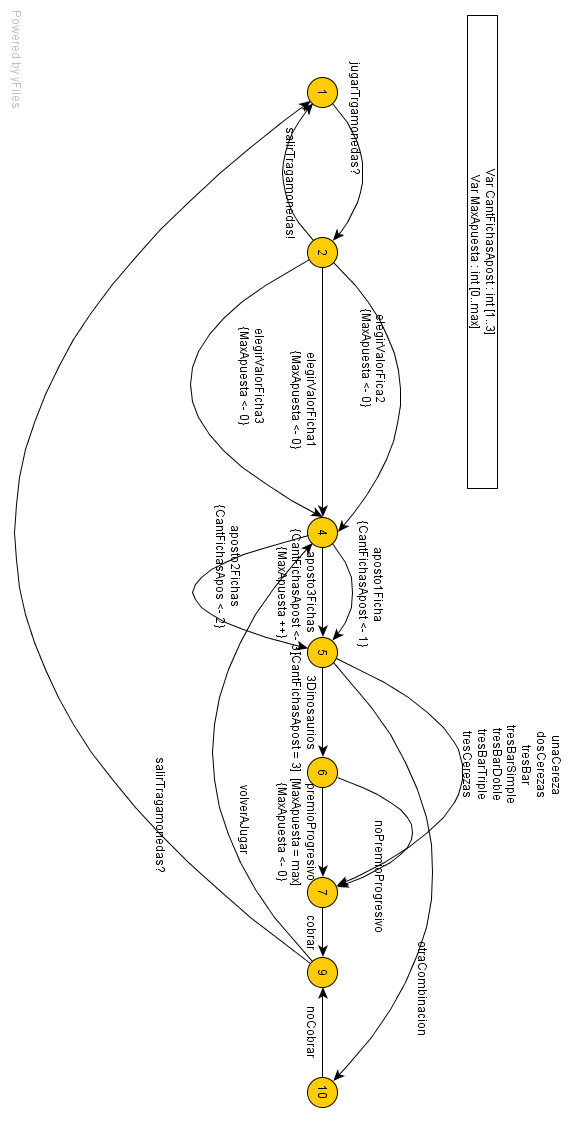
\includegraphics[scale=0.5]{img/JugadorTragamonedas.png}
\end{center}

Cada una de estas actividades se explican con mas detalle en los casos de uso: CU \jtra \ref{ljtra} y CU \apotra \ref{lapotra}

\begin{framed}

\depto Con esta maquina de estados finitos (FSM) mostramos el desarrollo del juego tragamonedas, modelando solo la parte de cobrar o no.

{\large FSM: JugadorTragamonedas}
\begin{center}
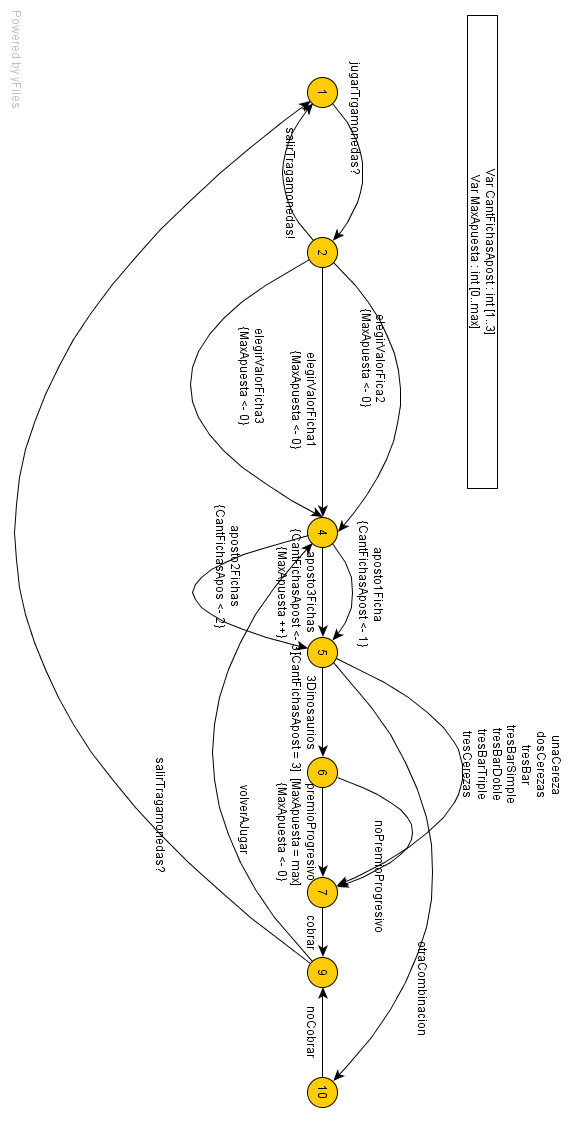
\includegraphics[scale=0.5]{img/JugadorTragamonedas.png}
\end{center}

\end{framed}

\subsection{Juego Craps}

Otro de los juegos elegidos por los socios es el \textbf{Craps}. En este juego un tirador lanza un par de dados para establecer un PUNTO y las apuestas girar�n en base a las posibilidades de que dicho tirador repita el mismo punto antes de lanzar un 7.
Cuando un jugador Craps decida jugar debe seleccionar una mesa existente o abrir una nueva. Luego durante el juego podra tirar los dados y/o apostar.

En el siguiente Diagrama de actividades se puede observar a grandes rasgos las actividades que realiza un jugador de craps.

\textcolor{red}{DADADADADADADADADA imagen repe}
\begin{figure}[h]
	\centering
		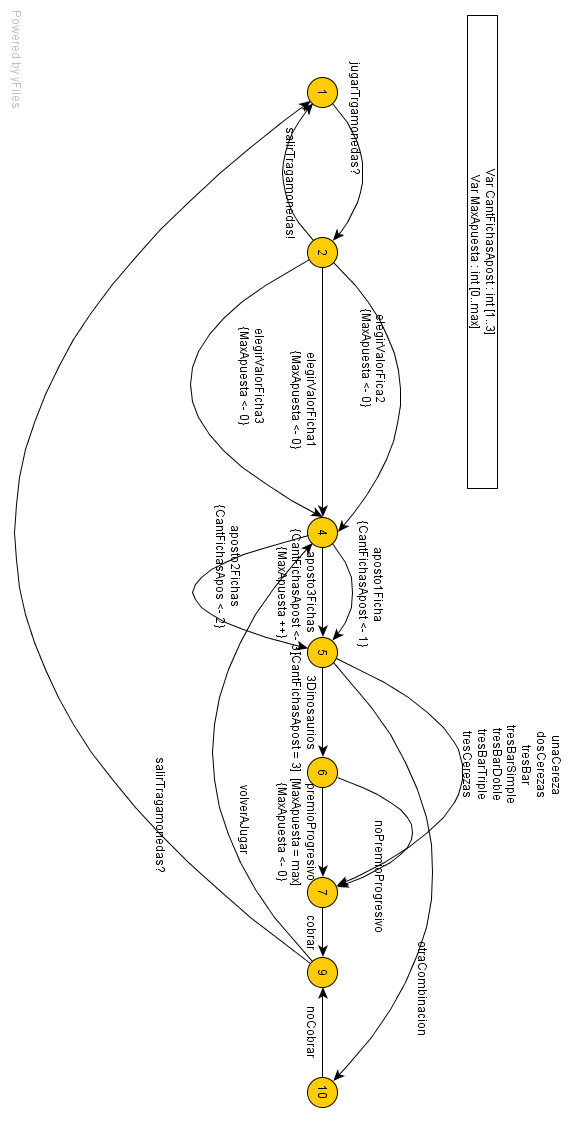
\includegraphics[scale=0.5]{img/JugadorTragamonedas.png}
	\caption{Diagrama de actividades Jugador Tragamonedas\label{fig:JugadorCraps}}
\end{figure}

Cada una de estas actividades se explican con mas detalle en los casos de uso: \\
CU \incr \ref{lincr}, CU \jcr \ref{ljcr}, \textcolor{red}{ referencia apo} y CU \scr \ref{lscr}




\begin{framed}

\depto Con estas maquinas de estados finitos (FSM) mostramos el desarrollo del juego craps. Incluyendo entre ellas un seleccionador, un tirador y cada una de las apuestas. 

{\large FSM: Seleccionador}
\begin{center}
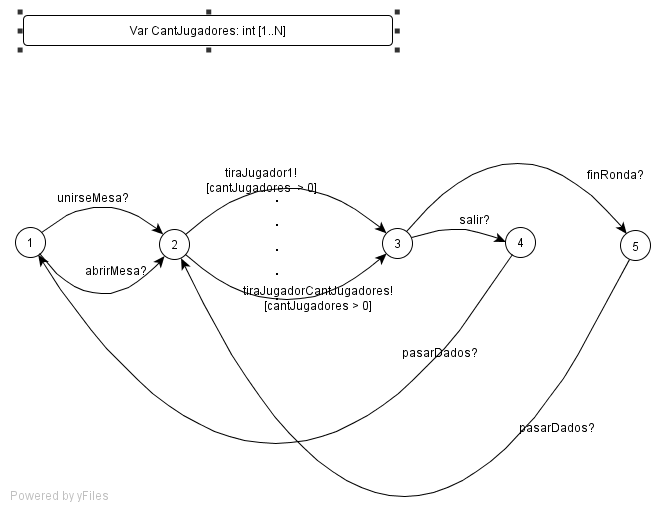
\includegraphics[scale=0.4]{img/seleccionador.png}
\end{center}

{\large FSM: Tirador}
\begin{center}
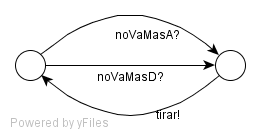
\includegraphics[scale=0.5]{img/tirador.png}
\end{center}

{\large FSM: Desarrollo Craps}
\begin{center}
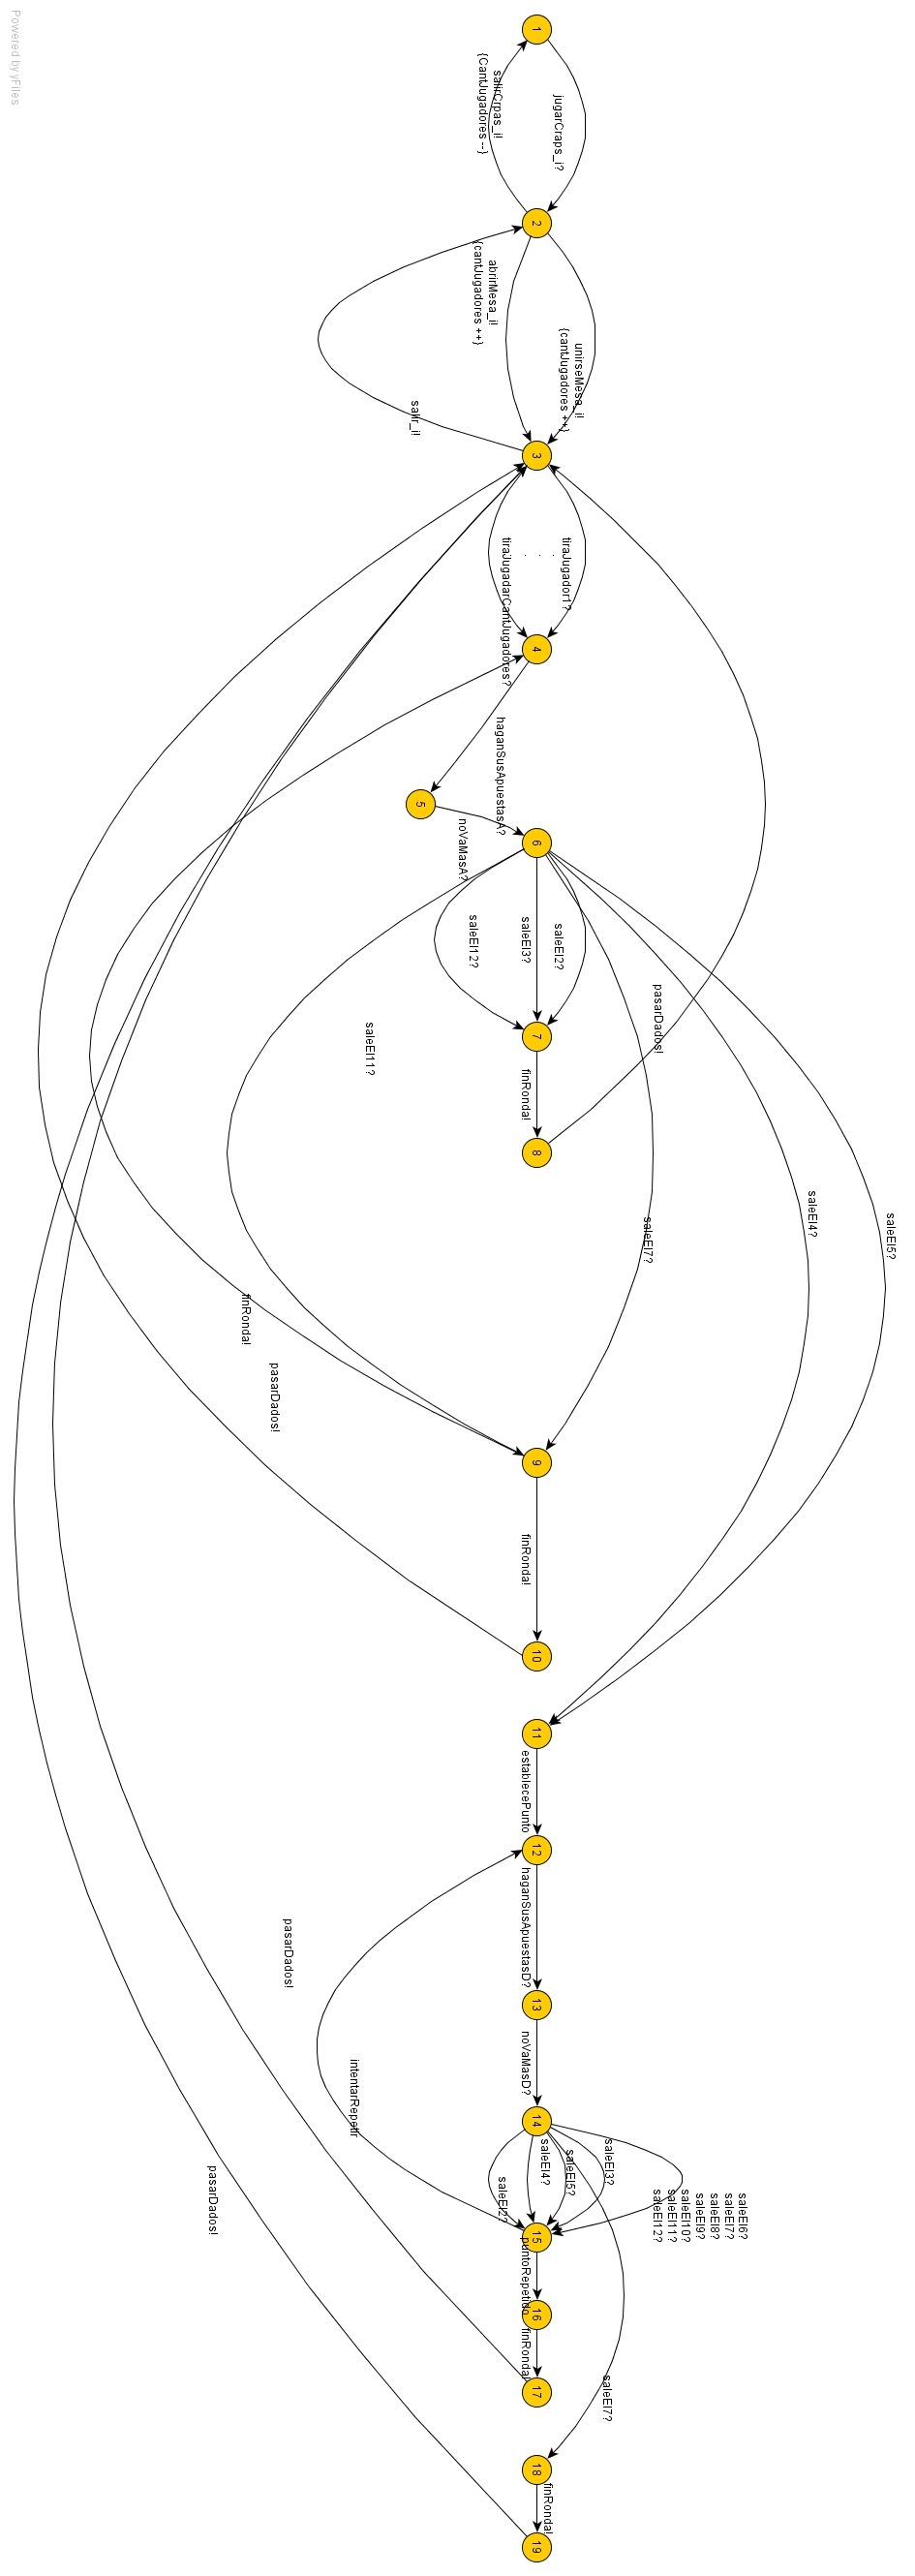
\includegraphics[scale=0.25]{img/desarrolloCraps.png}
\end{center}

\end{framed}















\subsection{Pago de jugadas y premios}

Se explicaran aqui con detalle como se refleja el pago de apuestas en el modelo propuesto (Modelo de Clases)\\
\textbf{NOTA: } Esta seccion esta dirigida a solo a lectores con conocimientos de modelo de clases conceptuales y OCL. 

\subsubsection{Pago de una jugada tragamonedas}

\begin{framed}

\depto Notese que una jugada tragamonedas solo tiene una apuesta que resolver.


\lstset{language=ocl}
\lstset{commentstyle=\textit}
\begin{lstlisting}[frame=trbl]{}

-- esta operacion paga la apuesta de una jugada de tragamonedas
-- dicha apuesta tiene que estar activa (de otro modo ya ha sido 
-- pagada) 
-- Se paga la jugada y se cobran los premios correspondientes
pagarJugadaTraga(j:JugadaTragamonedas):void
pre: j.estado = EstadoAp:activa
post: 
  -- pago resultado jugada y pago pozo progresivo 
  --y reseteo pozo progresivo
  pagarJugadaTragaBasica(j)
  -- cobro porcentaje jugada todos ponen
  cobrarJugadaToposPonen(j)
  -- pago jugada feliz y reseteo pozo feliz
  pagarJugadaFeliz(j)
  
  if damePremioTraga(j) <> 0
  then 
    j.estado = EstadoAp:Ganada
  else
    j.estado = EstadoAp:Perdida
    
  j.apuestaTragamonedas.retribucion = 
      j.hechaPor.saldo - j.hechaPor.saldo@pre


-- si la jugada es todos ponen decremento saldo jugador e 
-- incremento pozo feliz
pagarJugadaFeliz(j:JugadaTragamonedas):void
pre:  j.estado = EstadoAp:activa
post:   let tipoJugada = j.tipoDeJugada

  if tipoJugada.oclisTypeOf(Feliz)
    j.hechaPor.saldo = j.hechaPor.saldo@pre + 
        oclAsType(Feliz).pozoFeliz.monto
    oclAsType(Feliz).pozoFeliz.monto = 0
  endif


-- si la jugada es todos ponen decremento saldo 
-- jugador e incremento pozo feliz
cobrarJugadaToposPonen(j:JugadaTragamonedas):void
pre:  j.estado = EstadoAp:activa
post:  let tipoJugada = j.tipoDeJugada

  if tipoJugada.oclisTypeOf(TodosPonen)
  then 
    j.hechaPor.saldo = 

      j.hechaPor.saldo@pre +
      (damePremioTraga(j) + damePremioProgesivo(j)) * 
      100 / oclAsType(TodosPonen).porcentaje
    
    oclAsType(TodosPonen).pozoFeliz.monto = 

      oclAsType(TodosPonen).pozoFeliz.monto@pre + 
      ((damePremioTraga(j) + damePremioProgesivo(j)) * 
      100 / oclAsType(TodosPonen).porcentaje)
      
  endif



-- incremento saldo jugados de jugada y pozo progresivo 
-- (si corresponde)
-- decremento saldo casino
-- decremento pozo (si corresponde)
pagarJugadaTragaBasica(j:JugadaTragamonedas):void
pre:  j.estado = EstadoAp:activa
post:  
  let jornada = Jornada.allInstances->asSecuence->first()

  j.hechaPor.saldo = j.hechaPor.saldo@pre + 
       (damePremioTraga(j) + damePremioProgesivo(j))
  jornada.saldo = jornada.saldo@pre - cualEsElPrepmio(j)
  if damePremioProgesivo(j) <> 0
  then
    PozoProgresivo.allInstances()->asSecuence()->first().monto = 0
  endif


-- devuelve el valor del premio correspondiente a la jugada
damePremioTraga(j:JugadaTagamonesas):Numero
pre:  
post:  let conjRes:Collection  = 
ResultadoPosibleTagamonedas.allInstances()->select(  r |   
            r.res1 = j.res1 and
            r.res2 = j.res2 and
            r.res3 = j.res2 and
            r.cantMonedas = j.apuestaTragamonesas.cantMonedas) 
  let precioFicha = j.mesaTragamonedas.valorFicha

  if not(conjRes->isEmpty()) then
    result = conjRes->asSecuence()->first().ganMonedas * precioFicha 
  else
    result = 0

  endif 


-- devuelve el valor del premio progresivo 
-- correspondiente a la jugada
damePremioProgesivo(j:JugadaTagamonesas):Numero
pre:  true
post:  let conjRes:Collection  = 
ResultadoPosibleTagamonedas.allInstances()->select(r | r.res1 = j.res1 and
            r.res2 = j.res2 and
            r.res3 = j.res2 and
            r.cantMonedas = j.apuestaTragamonesas.cantMonedas) 
  let precioFicha = j.mesaTragamonedas.valorFicha

  if not(conjRes->isEmpty()) then
    if   j.res1 = Fruta::Dinosaurio and
      j.res2 = Fruta::Dinosaurio and
      j.res3 = Fruta::Dinosaurio and
      j.mesaTragamonedas.CantPalancasMax = 3
    then
      result = 
          j.mesaTragamonedas.pozoProgresivo.monto * precioFicha 
    else
      result = 0
    endif
  else
    result = 0
  endif 
  
\end{lstlisting}

\end{framed}